\section{Datasets and Tasks} \label{sec:datasets-tasks}

We conduct experiments on two datasets, the details for which are given below.

\subsection{Yelp Service Reviews}

We use a Yelp review dataset \citep{challenge2013yelp}, which has been sourced from the code repository accompanying the implementation of the paper by \cite{shen2017style}, open-sourced by the authors~\footnote{\url{https://github.com/shentianxiao/language-style-transfer}}. It contains 444101, 126670 and 63483 sentences for train, validation, and test, respectively, each sampling accompanied by binary sentiment labels. The maximum sentence length is 15, and the vocabulary size is about 9200.

\subsection{Amazon Product Reviews}

We also use an Amazon product reviews dataset~\footnote{\url{http://jmcauley.ucsd.edu/data/amazon/}}, following \cite{fu2017style}. The reviews were sourced from the code repository accompanying the paper~\footnote{\url{https://github.com/fuzhenxin/text_style_transfer}}. It contains 559142, 2000 and 2000 sentences for train, validation, and test, respectively, each sampling accompanied by binary sentiment labels. The maximum sentence length is 20, and the vocabulary size is about 58000.


\section{Implementation Details and Hyperparameters}

We implement the neural-network model in Tensorflow \citep{abadi2016tensorflow}, and use Scikit-learn \citep{pedregosa2011scikit}, NumPy and SciPy for evaluation metrics.

One of the most challenging aspects of training a variational autoencoder (VAE) is avoiding posterior collapse. In previous work \citep{yang2017improved, bowman2016generating, bahuleyan2017variational}, this has been done using manually crafted annealing schedules for weight of the KL divergence term. We utilize the $\tanh$ annealing schedule proposed by \cite{bahuleyan2017variational}, and also use their technique of appending the latent vector ($[\bm s; \bm c]$) to the hidden state of the recurrent decoder at each time-step of decoding.

We initialize the word embeddings matrix using pre-trained Word2Vec word embeddings \citep{mikolov2013efficient,mikolov2013distributed,mikolov2013linguistic} on each of the training corpora, which is then used for the autoencoder model. Greedy decoding  is used to predict the next word at each time-step of the decoder RNN \citep{germann2003greedy}.

The model uses style embeddings of size $8$ and content embeddings of size $128$ by default. The encoder and decoder are both GRU-RNNs with a size of $256$. The recurrent dropout probability for units in the encoder and decoder is $0.2$, and the same dropout probability is used for units in fully-connected layers as well.

We use the Adam optimizer \citep{kingma2014adam} for the autoencoder and the RMSProp optimizer \citep{tieleman2012lecture} for the discriminators, with an initial learning rate of $10^{-3}$, and train the model for 20 epochs. Both the autoencoder and the discriminators are trained once per epoch with $\lambda_\text{mult} = 1$, $\lambda_\text{adv} = 0.3$ and $\lambda_\text{badv} = 0.001$. For the VAE model, we set $\lambda_{\text{skl}} = 0.03$ and $\lambda_{\text{ckl}} = 0.03$.


\section{Evaluation Metrics} \label{sec:evaluation-metrics}

\subsection{Transfer Strength}

Transfer strength can be defined as a measure of how successful the model has been in generating sentences that are consistent with the attribute that needs to be transferred into them. This can be formulated as a Natural Language Understanding (NLU) task that takes in a sentence as input and predicts the probability of the presence of an attribute that we wish to evaluate the presence of.

Consistent with the approach taken by \cite{hu2017toward,shen2017style,fu2017style}, we train a separate model that learns to predict the label among the different labels to which transfer is possible. We use an open source implementation of the work presented by \cite{kim2014convolutional}, which is a convolutional neural network (CNN) model used for text classification \footnote{\url{https://github.com/dennybritz/cnn-text-classification-tf}}. This model has frequently been used as a text classification baseline to compare specialized models against \citep{tai2015improved,kiros2015skip,zhang2015character}. This CNN classifier is trained on the entire corpus described in the previous section, with a held out validation dataset to assess improvements in accuracy over time. The test dataset for this classifier consists of the style-transferred sentences generated from the autoencoder model.

The style transfer strength is the ratio of sentences successfully transferred to the target style, to the total number of test sentences.
\begin{equation*}
	\text{transfer-strength} = \frac{count(\text{generated sentences with target style attribute})}{count(\text{generated sentences})}
\end{equation*}

Therefore, the optimal style transfer strength score is 1 and the worst is 0. Here, we choose to ignore the classification errors by our automated classification model, since a good model (with a high classification accuracy) would mis-classify an approximately equal number of samples for each label, and a biased classifier would negatively impact the style transfer strength score. This metric measures the sentence-level style transfer i.e. if 90 sentences are transferred out of 100, the transfer strength is 0.9.

The classifier we train achieves a classification accuracy of approximately $0.97$ on the Yelp validation data, and $0.84$ on the Amazon validation data.

\subsection{Content Preservation} \label{ssec:content-preservation-metric}

The content preservation metric used by \cite{fu2017style} is also used in our work to judge content preservation of the generated sentences compared to the original. This metric is required to ensure that the generated sentences don't contain content, subjects or topics entirely different compared to the original sentences. It measures the sentence-level content preservation.

This method uses 100-dimensional GloVe embeddings \citep{pennington2014glove} pre-trained on the Wikipedia + GigaWord corpora~\footnote{\url{https://nlp.stanford.edu/projects/glove/}}. The min, mean and max GloVe word embeddings for each sentence are concatenated together to create a sentence representation. The cosine similarity between the source sentence and target sentence is used as a measure of content preservation.

Let $W$ be the set of word embeddings in any sentence $s$. Then the cosine similarity between two sentences $s_1$ and $s_2$ is obtained by
\begin{align*}
	\text{emb} =
	 & [min(W);max(W);mean(W)]              \\
	\text{cosine-similarity} =
	 & 1 - \cos(\text{emb}_1, \text{emb}_2)
\end{align*}
where $\text{emb}_1$ and $\text{emb}_2$ are the sentence embeddings for $s_1$ and $s_2$ respectively. The mean cosine similarity of all the sentences in the test dataset is the content preservation that is reported for the experiment.

\begin{table}[ht]
	\centering
	\begin{tabular}{| p{0.45\linewidth} | p{0.45\linewidth} |}
		\hline
		\tabc{1}{Original (Positive)}                                                       & \tabh{Transferred (Negative)}                    \\
		\hline
		\hline
		we had the shrimp with vegetables and shrimp fried rice both lovely                 & we had the bacon cheeseburger and it was cold    \\
		\hline
		both dishes prepared with quality veggies                                           & eggs benedict with no flavor                     \\
		\hline
		my appetizer was also very good and unique                                          & my steak was very dry and flavorless             \\
		\hline
		both times i have eaten the lunch buffet and it was outstanding                     & yes i have had the worst pizza i have ever had   \\
		\hline
		the new york eggrolls are outstanding and the beef dishes we ordered were flavorful & the main issue was our server was extremely rude \\
		\hline
		\hline
		\tabc{1}{Original (Negative)}                                                       & \tabh{Transferred (Positive)}                    \\
		\hline
		\hline
		the chicken '' strip were paper thin oddly flavored strips                          & the bread was wonderful as well                  \\
		\hline
		the big chicken sandwich should be called the big mayonnaise sandwich               & the salsa is the best i have ever had            \\
		\hline
		fries are not worth coming back                                                     & prices are good                                  \\
		\hline
		but honestly the worst hookah in las vegas                                          & very authentic food in the east valley           \\
		\hline
		second the service was terribly slow                                                & the sushi was delicious                          \\
		\hline
	\end{tabular}
	\caption{Examples of Poor Content Preservation}
	\label{tab:poor-content-preservation}
\end{table}

As seen in the examples in Table \ref{tab:poor-content-preservation}, it is easy to optimize for a style-transfer objective as long as there are no constraints on the content preservation regularization. However, this results in a disconnect in terms of content and the generated sentence no longer resembles the original. To ensure this does not happen, we typically use a much larger content latent space than style latent space, as well as add the necessary regularizations discussed in the previous chapter. Similar to \cite{fu2017style}, for the sentiment task, we exclude words from a sentiment lexicon \citep{hu2004mining} while evaluating the content preservation score.

However, a slight drawback of this content preservation metric devised by \cite{fu2017style} is that it takes a small range of possible values, and is therefore less sensitive to model performance changes. In theory, the maximum content preservation value achievable is 1 and the minimum is 0. However, from experiments performed by matching random pairs of Yelp corpus sentences, the content preservation we observe is $0.7591 \pm 0.0004$. This can be treated as an approximate lower bound on the metric for model assessment.

\subsection{Word Overlap}

In addition to the content preservation metric described above, we also utilize a simpler unigram overlap metric. Given a source sentence $x$ and an attribute style transferred sentence $y$, let $w_x$ and $w_y$ be the set of unique words present in $x$ and $y$ respectively. Then, the word overlap score can be calculated using
\begin{equation*}
	\text{word-overlap} = \frac{count(w_x \cap w_y)}{count(w_x \cup w_y)}
\end{equation*}
which is simply a normalized measure of overlapping unigrams in the source and target sentences, aggregated over all the sentences being evaluated.

Theoretically, the word overlap score ranges from 0 to 1. However, in practice, since the expectation is that some words will be changed due to the style-transfer process, we wish to strike a good balance with respect to the style transfer strength and original content preservation. Using experiments on random pairs of sentences, the word overlap score computed is $0.0098 \pm 0.0006$, which can again be treated as a more realistic approximate lower-bound on this metric.

Word overlap can be used interchangeably with the `Content Preservation' metric described above. For the experiments in this work, we report both.


\subsection{Language Fluency}

Previous works in this area have either utilized human evaluations \citep{shen2017style,fu2017style} to evaluate language fluency and content preservation, or do not evaluate it at all \citep{hu2017toward}.

We use a trigram based Kneser–Ney Smoothed language model \citep{kneser1995improved} as a quantifiable and automated scoring metric by which to assess the quality of generated sentences. It calculates the probability distribution of trigrams in a document based on their occurrence statistics to build a language model. We train this language model on the complete corpus that we evaluate our style transfer models with. This metric is a word-level evaluator of the fluency of the generated sentences, aggregated over all the sentences.

After the generation of style transferred sentences, we parse them out into trigrams, and calculate the probabilities of each of the trigrams being from the same corpora as the original model was trained on. The log-likelihood scores, as predicted by the Kneser-Ney language model and aggregated over the generated corpus, are reported as the indicator for language fluency.


\subsection{A Note about Cycle Consistency Loss}

The cycle consistency loss is described in the image domain-adaptation work done by \cite{zhu2017unpaired}. Given domains $X$ and $Y$, they aim to learn a mapping similar to ours, $G: X \rightarrow Y$ which transfers attributes of $X$ to $Y$. At the same time, they also learn an inverse mapping $F: Y \rightarrow X$. The cycle consistency loss is the step that pushes $F(G(X)) \approx X$ and $G(F(Y)) \approx Y$, as shown in Figure \ref{fig:cycle-consistency}.

\begin{figure}[ht]
	\centering
	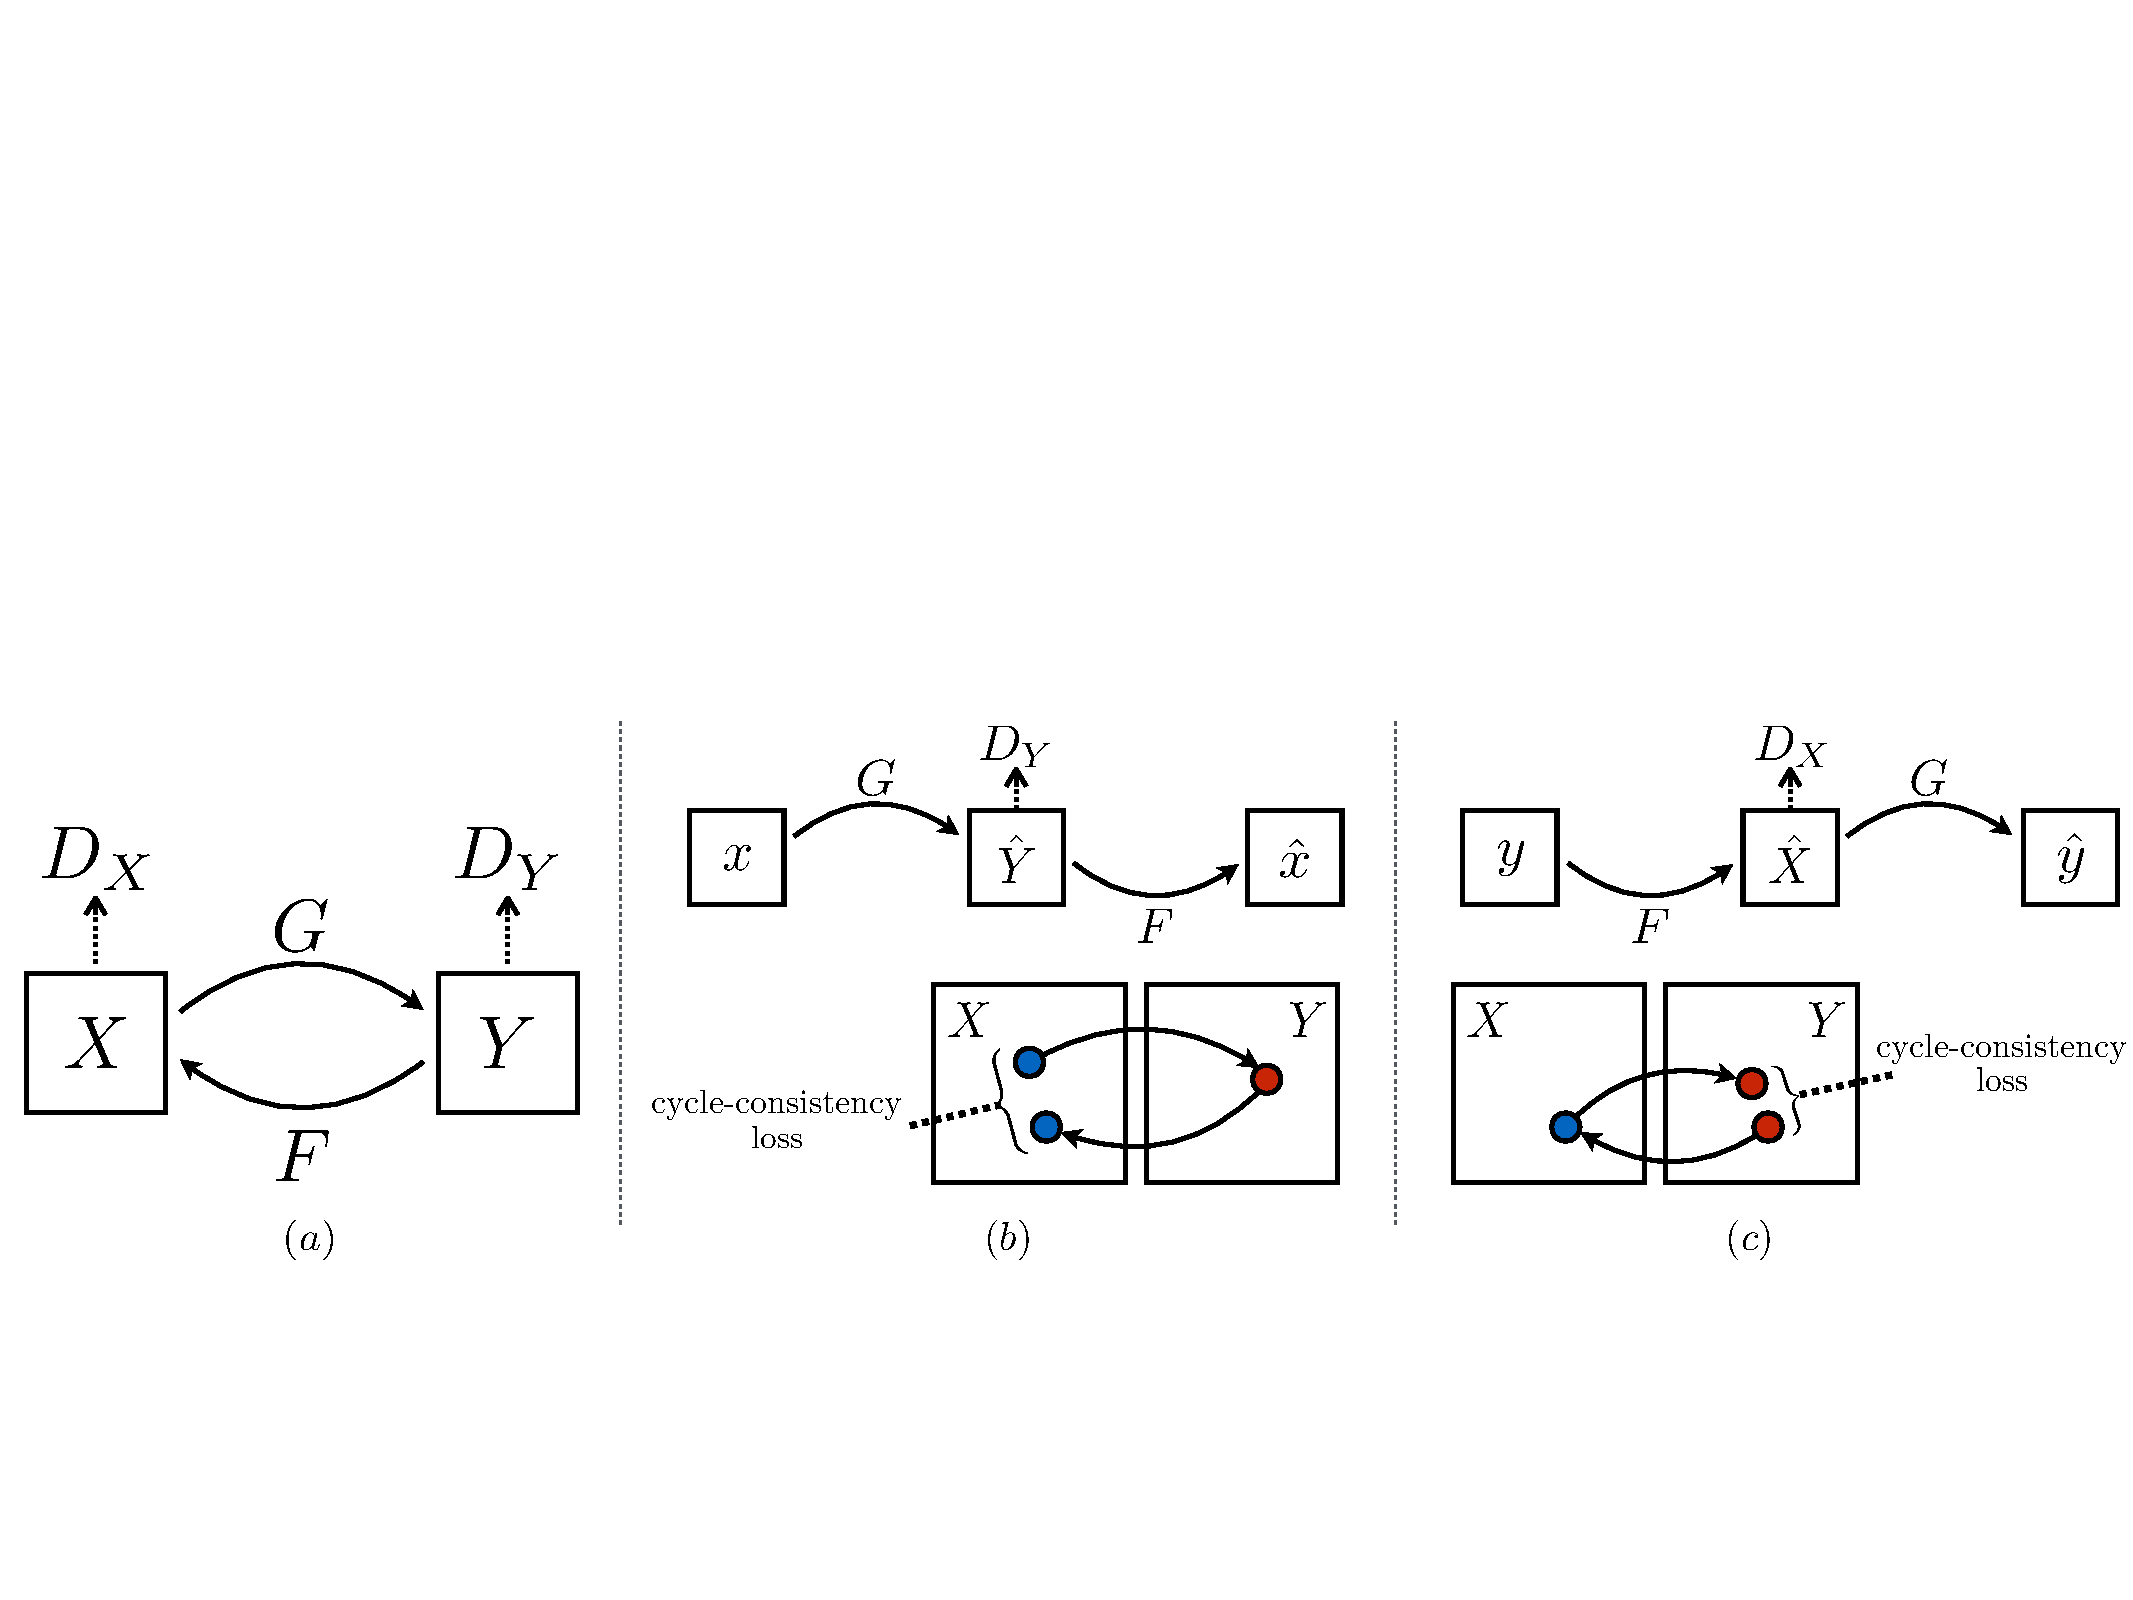
\includegraphics[width=\textwidth]{images/cycle-consistency}
	\imgsrc{\cite{zhu2017unpaired}}
	\caption{\label{fig:cycle-consistency} Cycle Consistency Loss}
\end{figure}

This training routine could also be used as an evaluation metric for other domain adaptation tasks, like text attribute style transfer. The advantage of using a cycle consistency loss is that no other content preservation metric is needed, and no domain or style specific lexicons would be needed.

In the case of our model, assume that, for a sample sentence $x$ from the domain $X$ and the ideal equivalent sentence transferred to the domain $Y$ is $y$. The transferred sentence generated by our model is $\hat{y}$. In the previous approaches, we compare $\hat{y}$ with the original $x$ using a content similarity metric. However, if the cycle consistency loss were to be used, we can further transfer the style of the sentence $\hat{y}$ back to the domain $X$, obtaining $\hat{x}$. Now that we have two sentences in the same domain i.e. $x$ and $\hat{x}$, it is a lot simpler to compare them, and this can be achieved by traditional parallel corpora evaluation metrics like BLEU \citep{papineni2002bleu}.

However, in our problem, a scenario in which both functions $F$ and $G$ do not successfully disentangle style and content, like the examples presented in Table \ref{tab:poor-content-preservation}, is a possibility. This results in the undesirable transfer of content, in addition to the desired transfer of style at inference time. In this case, the transformation could look like
\begin{equation*}
	x \xrightarrow{G} y^* \xrightarrow{F} x
\end{equation*}
where $y^*$ is a sentence with the requisite transferred style, as well as undesirable transferred content. Such examples would score highly on both the style transfer strength metric and the cycle consistency metric, while still producing generated sentences of poor quality i.e. generated sentences with changed content.

Hence, this metric would not be able to tell the difference between a model with poor content preservation and a good model, and we refrain from using it in our evaluation.


\section{Experiment Results}

\subsection{Disentangling Latent Space}

We first analyse how the style (sentiment) and content of the latent space are disentangled. We train softmax classifiers that use each set of latent space units as features. These classifiers are trained alongside the autoencoder model - without updating the encoder parameters - to predict the true class of an input sample. The results reported here are for the Yelp dataset and are shown in Table \ref{tab:latent-space-classification}.

\begin{table}[ht]
	\centering
	\begin{tabular}{| l | r | r |}
		\hline
		                                        & \tabh{DAE}                  & \tabh{VAE} \\
		\hline \hline
		Random/Majority guess                   & \multicolumn{2}{c|}{0.6018}              \\ \hline \hline
		Content latent space  ($\bm c$)         & 0.6137                      & 0.6567     \\ \hline
		Style latent space ($\bm s$)            & 0.7927                      & 0.7911     \\ \hline
		Complete latent space ($[\bm s;\bm c]$) & 0.7918                      & 0.7918     \\
		\hline
	\end{tabular}
	\caption{Results - Style Classification Accuracy}
	\label{tab:latent-space-classification}
\end{table}

The latent space can also be visualized with our method since we are able to infer a pair of style and content embeddings for every training data sample. We use t-SNE plots \citep{maaten2008visualizing} and use a set of random samples from each label to plot both the style and content embeddings inferred for them during a given epoch of the training procedure. Our hypothesis is that while the points for different labels plotted in the content embedding space would be mixed and indistinguishable in terms of plot co-ordinates, the style embedding space would display the opposite characteristic and show a clean separation of representative samples for each label.

We show t-SNE plots of both the deterministic autoencoder (DAE) and the variational autoencoder (VAE) models in Figure \ref{fig:dae-tsne} and Figure \ref{fig:vae-tsne}, respectively.

\begin{figure}[ht]
	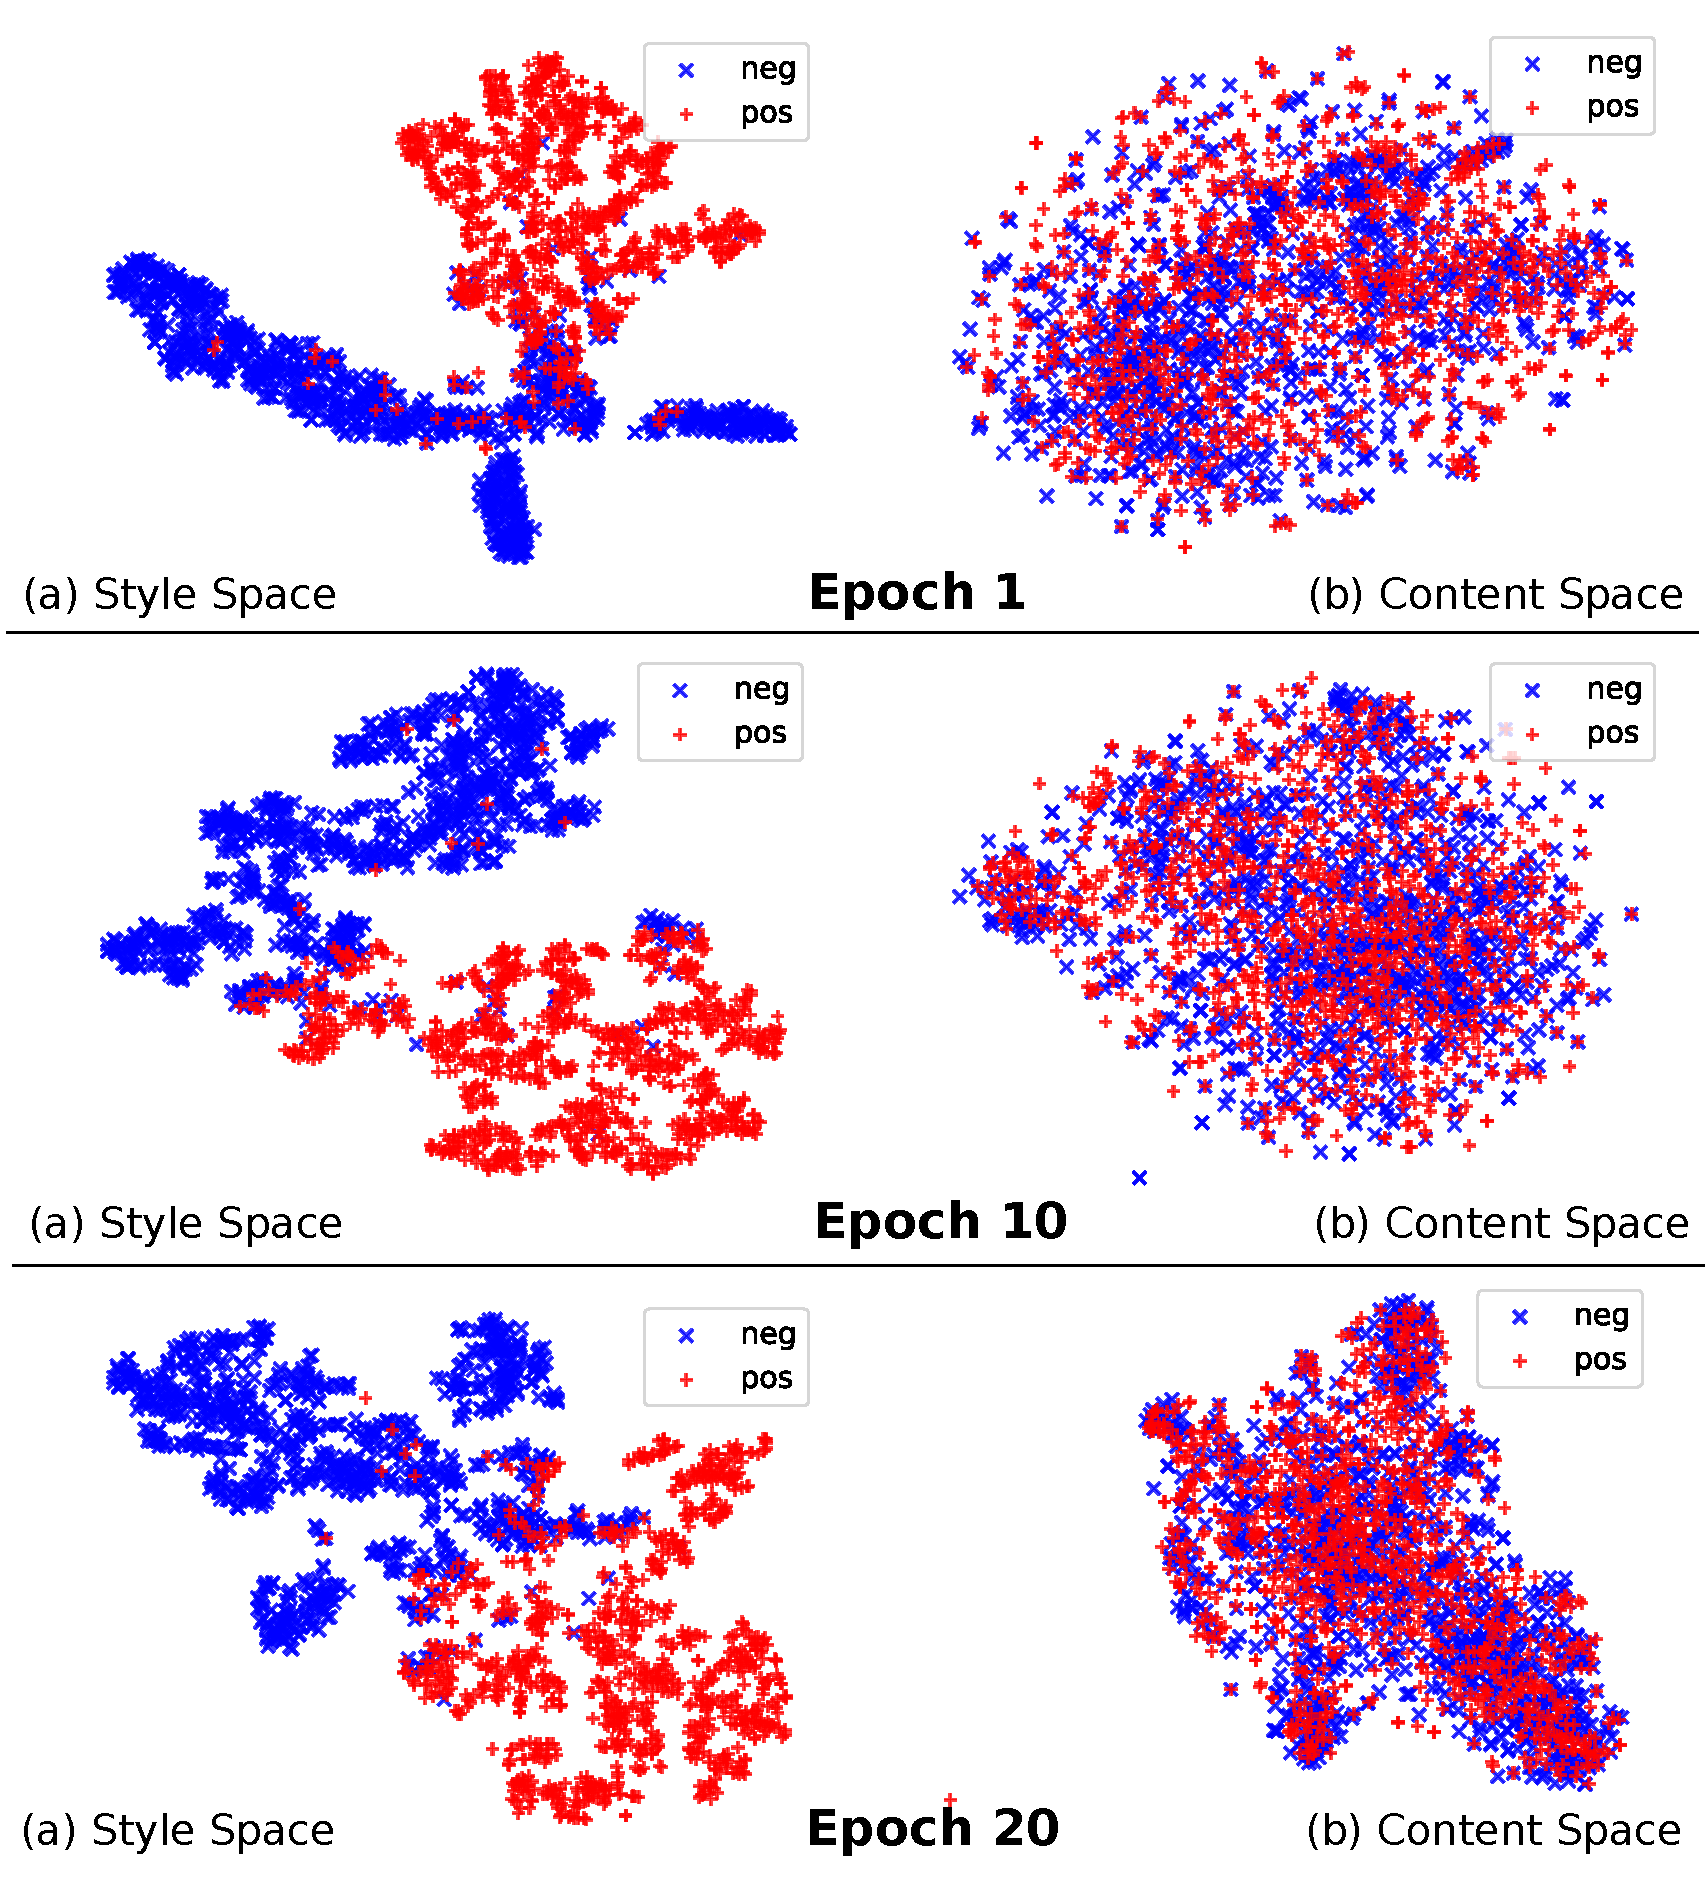
\includegraphics[width=\linewidth]{images/latent-spaces-dae}
	\caption{T-SNE Plots: (a) Style and (b) Content Spaces - DAE Model}
	\label{fig:dae-tsne}
\end{figure}

\begin{figure}[ht]
	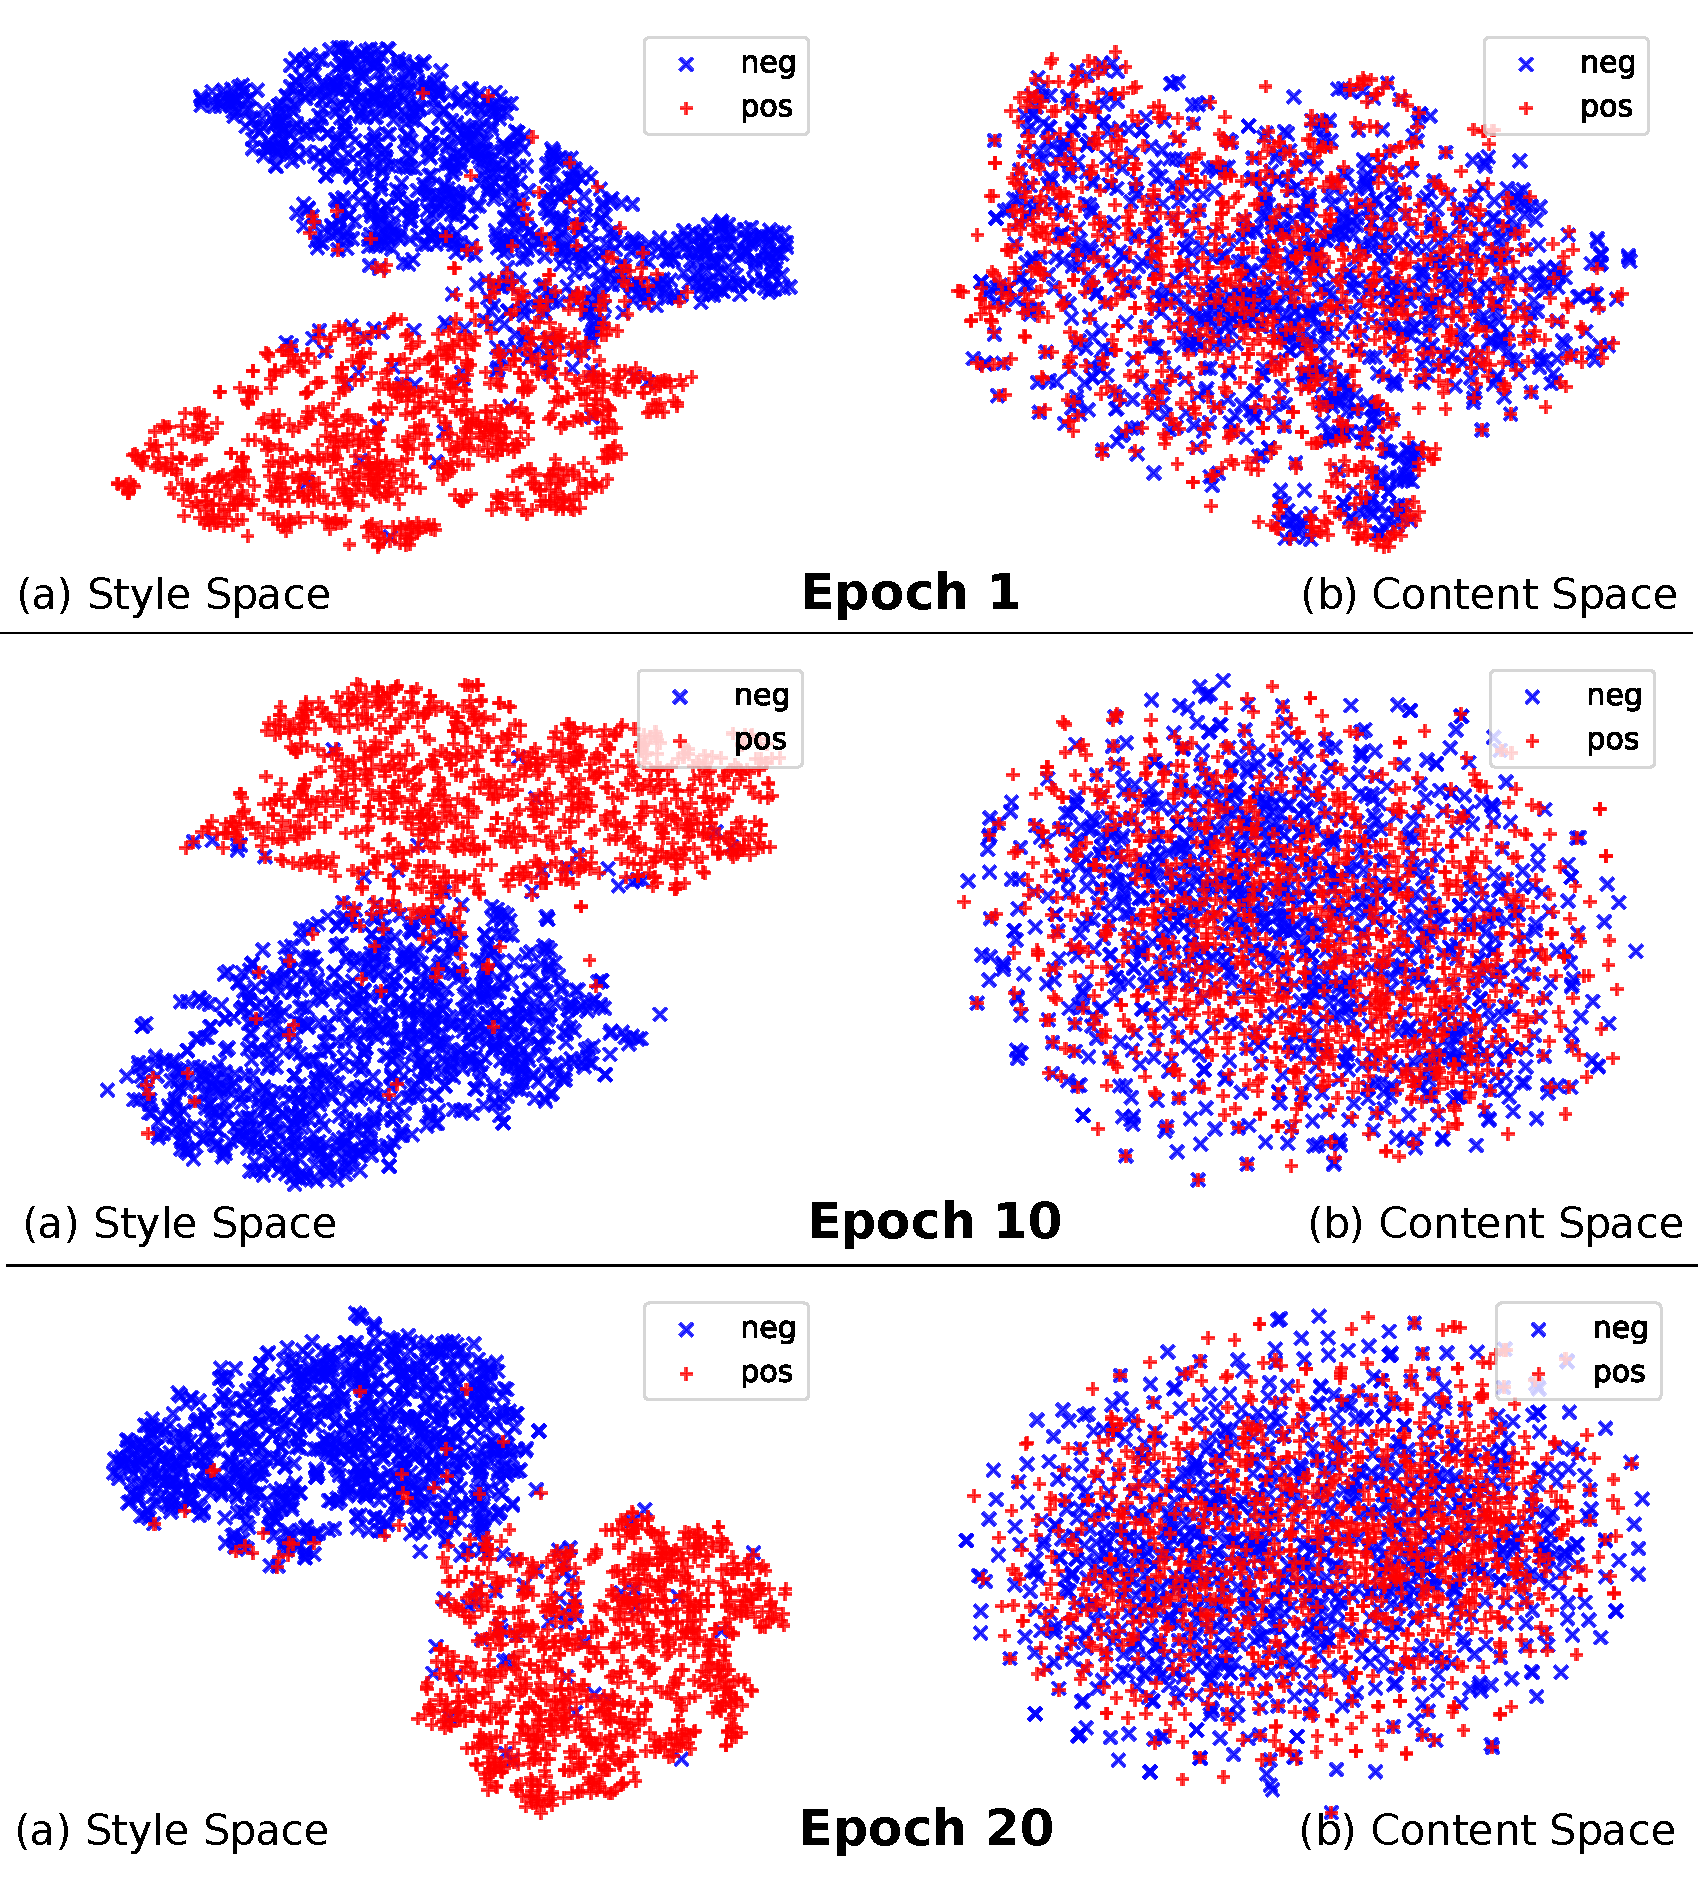
\includegraphics[width=\linewidth]{images/latent-spaces-vae}
	\caption{T-SNE Plots: (a) Style and (b) Content Spaces - VAE Model}
	\label{fig:vae-tsne}
\end{figure}

\subsection{Style-Transferred Text Generation}

We apply our model to a style-transfer sentence generation task, where the goal is to generate a sentence with different sentiment (interpreted as style in this task). We use the metrics discussed in Section \ref{sec:evaluation-metrics} to evaluate our models.

We compare our approach with the current state-of-the-art work in automated text attribute style transfer \citep{shen2017style,fu2017style}. We re-conduct the experiments using their publicly available code and the datasets described in Section \ref{sec:datasets-tasks}. The results are shown in Table \ref{tab:comparison-previous} (Yelp dataset) and Table \ref{tab:comparison-previous-ama} (Amazon dataset). The models used for evaluations on both datasets are identical.

\begin{table}[ht]
	\centering
	\begin{tabular}{| l | r | r | r | r |}
		\hline
		\tabc{2}{Model}                       & \tabh{Transfer} & \tabh{Content}      & \tabh{Word}    & \tabh{Language} \\
		                                      & \tabh{Strength} & \tabh{Preservation} & \tabh{Overlap} & \tabh{Fluency}  \\
		\hline
		\hline
		Cross-Alignment \citep{shen2017style} & 0.8087          & 0.8920              & 0.2087         & -23.3886        \\
		\hline
		Style Embedding \citep{fu2017style}   & 0.1819          & 0.9586              & 0.6661         & -16.1711        \\
		\hline
		Ours (DAE)                            & 0.8425          & 0.8924              & 0.2552         & -16.4808        \\
		\hline
		Ours (VAE)                            & 0.8903          & 0.8824              & 0.2105         & -14.4099        \\
		\hline
	\end{tabular}
	\caption{Results - Yelp Dataset Sentiment Transfer}
	\label{tab:comparison-previous}
\end{table}

\begin{table}[ht]
	\centering
	\begin{tabular}{| l | r | r | r | r |}
		\hline
		\tabc{2}{Model}                       & \tabh{Transfer} & \tabh{Content}      & \tabh{Word}    & \tabh{Language} \\
		                                      & \tabh{Strength} & \tabh{Preservation} & \tabh{Overlap} & \tabh{Fluency}  \\
		\hline
		\hline
		Cross-Alignment \citep{shen2017style} & 0.6063          & 0.8933              & 0.0241         & -26.3093        \\
		\hline
		Style Embedding \citep{fu2017style}   & 0.4165          & 0.9332              & 0.3588         & -28.1346        \\
		\hline
		Ours (DAE)                            & 0.7032          & 0.9178              & 0.1305         & -32.4184        \\
		\hline
		Ours (VAE)                            & 0.7259          & 0.9090              & 0.0814         & -28.4953        \\
		\hline
	\end{tabular}
	\caption{Results - Amazon Dataset Sentiment Transfer}
	\label{tab:comparison-previous-ama}
\end{table}


Table \ref{tab:ablation-results} presents the results of ablation tests done by evaluating our model using all possible combinations of our training objectives. We see that both, the adversarial and multi-task losses, play a role in the strength of style transfer. It also shows that their usage in a combination can further boost performance of the style-transfer strength.

\begin{table}[ht]
	\centering
	\begin{tabular}{| l | r | r | r | r |}
		\hline
		\tabc{2}{Objectives}                                     & \tabh{Transfer} & \tabh{Content}      & \tabh{Word}     & \tabh{Language}   \\
		                                                         & \tabh{Strength} & \tabh{Preservation} & \tabh{Overlap}  & \tabh{Fluency}    \\
		\hline
		\hline
		$\loss{rec}$                                             & 0.1436          & \textbf{0.9154}     & \textbf{0.3288} & -14.2781          \\
		\hline
		$\loss{rec}$, $\loss{adv}$                               & 0.7274          & 0.8800              & 0.2037          & -14.1567          \\
		\hline
		$\loss{rec}$, $\loss{mult}$                              & 0.7894          & 0.8976              & 0.2589          & -14.5607          \\
		\hline
		$\loss{rec}$, $\loss{badv}$                              & 0.1677          & 0.9147              & 0.3282          & -14.4486          \\
		\hline
		$\loss{rec}$, $\loss{adv}$, $\loss{mult}$                & \textbf{0.8903} & 0.8824              & 0.2105          & -14.4099          \\
		\hline
		$\loss{rec}$, $\loss{adv}$, $\loss{badv}$                & 0.7491          & 0.8827              & 0.2022          & -14.3568          \\
		\hline
		$\loss{rec}$, $\loss{mult}$, $\loss{badv}$               & 0.7832          & 0.8958              & 0.2567          & -14.3373          \\
		\hline
		$\loss{rec}$, $\loss{adv}$, $\loss{mult}$, $\loss{badv}$ & 0.8846          & 0.8782              & 0.1970          & \textbf{-14.0479} \\
		\hline
	\end{tabular}
	\caption{Results - Ablation Tests}
	\label{tab:ablation-results}
\end{table}

Some qualitative examples of style-transferred sentence generation are presented in Table \ref{tab:transfer-samples}. We see that, with the empirically estimated style vector, we can flexibly control the sentiment of generated sentences.

\begin{table}[ht]
	\centering
	\begin{tabular}{| p{0.3\linewidth} | p{0.3\linewidth} | p{0.3\linewidth} |}
		\hline
		\tabc{2}{Original (Positive)}                          & \tabh{DAE Transferred}                                         & \tabh{VAE Transferred}                                      \\
		                                                       & \tabh{(Negative)}                                              & \tabh{(Negative)}                                           \\
		\hline
		i would recommend a visit here                         & i would not recommend this place again                         & i would not recommend this place for my experience          \\
		\hline
		the restaurant itself is romantic and quiet            & the restaurant itself is soooo quiet                           & the restaurant itself was dirty                             \\
		\hline
		my experience was brief but very good                  & my experience was very loud and very expensive                 & my experience was ok but not very much                      \\
		\hline
		the food is excellent and the service is exceptional   & the food is by the worst part is the horrible costumer service & the food was bland and i am not thrilled with this          \\
		\hline
		the food is very very amazing like beef and fish       & the food is very horrible i have ever had mostly fish          & the food is very bland and just not fresh                   \\
		\hline
		we will definitely come back here                      & we will not come back here again                               & we will never come back here                                \\
		\hline
		both were very good                                    & everything was very bland                                      & both were very bad                                          \\
		\hline
		\hline
		\tabc{2}{Original (Negative)}                          & \tabh{DAE Transferred}                                         & \tabh{VAE Transferred}                                      \\
		                                                       & \tabh{(Positive)}                                              & \tabh{(Positive)}                                           \\
		\hline
		\hline
		so nasty                                               & so helpful                                                     & so fabulous                                                 \\
		\hline
		consistently slow                                      & consistently awesome                                           & fast service                                                \\
		\hline
		crap fries hard hamburger buns burger tasted like crap & cheap and yummy sandwiches really something different          & yummy hamburgers and blue cheese bagels are classic italian \\
		\hline
		oh and terrible tea                                    & oh and awesome tea                                             & oh and great tea                                            \\
		\hline
		the interior is old and generally falling apart        & the interior is clean and orderly as entertaining              & the interior is old and noble                               \\
		\hline
		front office customer service does not exist here      & front office is very professional does you                     & kudos to customer service is very professional              \\
		\hline
		the crust was kinda gooey like                         & the crust is kinda traditional                                 & the crust is soooooo worth it                               \\
		\hline
	\end{tabular}
	\caption{Style-Transferred Text Examples}
	\label{tab:transfer-samples}
\end{table}


In this chapter, we have described the datasets and task, and presented quantitative results for the disentangled space learning and its application to a style (sentiment) transfer task. We also display qualitative results of sentences generated by our model. In the next chapter, we perform a deeper analysis for each result presented here. We also show trade-offs between model scores on different metrics and discuss methods whose results do not fit our original hypotheses.
